\documentclass[a4paper,11pt]{article}
\pdfoutput=1 % if your are submitting a pdflatex (i.e. if you have
             % images in pdf, png or jpg format)

\usepackage{jheppub} % for details on the use of the package, please
                     % see the JHEP-author-manual

\usepackage[T1]{fontenc} % if needed
\usepackage{framed}

\usepackage{dsfont}
\title{\boldmath Introduction to Conformal Field Theory}


%% %simple case: 2 authors, same institution
%% \author{A. Uthor}
%% \author{and A. Nother Author}
%% \affiliation{Institution,\\Address, Country}

% more complex case: 4 authors, 3 institutions, 2 footnotes


% The "\note" macro will give a warning: "Ignoring empty anchor..."
% you can safely ignore it.

%\affiliation[a]{One University,\\some-street, Country}


% e-mail addresses: one for each author, in the same order as the authors
%\emailAdd{first@one.univ}






\abstract{Abstract...}



\begin{document} 
\maketitle
\flushbottom
\newpage
\section{Introduction}

\section{Conformal Transformation in $d$-Dimensions}

Let $\mathcal{M}=\mathbb{R}^{p,q}$ be a manifold $\mathbb{R}^d$ with the metric
\begin{equation}
    g_{\mu\nu}=\eta_{\mu\nu}=\mathrm{diag}(1,1,...,1,-1,-1,....,-1).
\end{equation}
with $p$ copies of $1$ entries and $q$ copies of $-1$ entries where $p,q\in\mathbb{Z}^+$ and $d=p+q$.

Consider a smooth change of coordinate
\begin{equation}
    x\rightarrow x'=x'(x)
\end{equation}
such that
\begin{equation}
    g_{\mu\nu}\rightarrow g'_{\mu\nu}(x')=\frac{\partial x^\alpha}{\partial x'^\mu}\frac{\partial x^\beta}{\partial x'^\nu}g_{\alpha\beta}(x)
\end{equation}
where
\begin{equation}
    g'_{\mu\nu}(x')=\Omega(x')g_{\mu\nu}(x')\propto\eta_{\mu\nu}
\end{equation}
with $\Omega(x)>0$. Such a transformation is called conformal. Conformal transformations preserve angles, i.e.
\begin{equation}
    \angle\theta=\frac{g_\mu\nu u^\mu v^\nu}{\sqrt{(g_{\mu\nu} u^\mu v^\nu)^2}}.
\end{equation}
\begin{framed}
    The conformal group $\mathrm{Conf}(\mathcal{M})$ is the connected component containning the identity in the group of all conformal transformations of $\mathcal{M}$.
\end{framed}
\subsection{Classification of $\mathrm{Conf}(\mathbb{R}^{p,q})$ via Infinitesimal Argument}

Consider an infinitesimal conformal transformation
\begin{equation}
    x^\mu\rightarrow x^\mu+\epsilon^\mu(x).
\end{equation}
The change of metric is
\begin{equation}
\begin{aligned}
g'_{\mu\nu}&=\frac{\partial x^\alpha}{\partial x'^\mu}\frac{\partial x^\beta}{\partial x'^\nu}g_{\alpha\beta}\\
&=(\delta^\alpha_\mu-\partial_\mu\epsilon^\alpha)(\delta^\beta_\nu-\partial_\nu\epsilon^\beta)g_{\alpha\beta}\\
&=g_{\mu\nu}-(\partial_\mu\epsilon_\nu+\partial_\nu\epsilon_\mu)+\mathcal{O}(\epsilon^2)
\end{aligned}
\end{equation}
In order to satisfy $g'_{\mu\nu}\propto\eta_{\mu\nu}$, we need
\begin{equation}
    \partial_\mu\epsilon_\nu+\partial_\nu\epsilon_\mu\propto\eta_{\mu\nu}
\end{equation}
By taking the trace of above equation, we finally have
\begin{equation}
    \partial_\mu\epsilon_\nu+\partial_\nu\epsilon_\mu=\frac{2}{d}(\partial\epsilon)\eta_{\mu\nu}
    \label{1star}
\end{equation}
with $\Omega(x)=1+\frac{2}{d}(\partial\epsilon)$.

A direct result from Eq.(\ref{1star}) is 
\begin{equation}
    [\eta_{\mu\nu}\Box+(d-2)\partial_\mu\partial_\nu](\partial\epsilon)=0
    \label{1starstar}
\end{equation}
The steps lead to above result are shown as below


\begin{framed}
By acting $\partial_\rho$ on Eq.(\ref{1star}) and permute indexes $\mu$, $\nu$ and $\rho$, we have
\begin{equation}
\begin{aligned}
\partial_\rho\partial\mu\epsilon_\nu+\partial_\rho\partial_\nu\epsilon_\mu=\frac{2}{d}\partial\rho(\partial\epsilon)\eta_{\mu\nu}\\
\partial_\mu\partial\rho\epsilon_\nu+\partial_\mu\partial_\nu\epsilon_\rho=\frac{2}{d}\partial\mu(\partial\epsilon)\eta_{\mu\nu}\\
\partial_\nu\partial\rho\epsilon_\mu+\partial_\nu\partial_\mu\epsilon_\rho=\frac{2}{d}\partial\nu(\partial\epsilon)\eta_{\mu\nu}
\end{aligned}.
\end{equation}
Use the summation of last 2 equations to subtract the first one, we get
\begin{equation}
    2\partial_\mu\partial_\nu\epsilon_\rho=\frac{2}{d}(\eta_{\rho\mu}\partial_\nu+\eta_{\rho\nu}\partial_\mu-\eta_{\mu\nu}\partial_\rho)(\partial\epsilon).
\end{equation}
By acting $\partial^\rho$ to above equation, we finally have the result in Eq.(\ref{1starstar})
\end{framed}
\subsubsection{$d>2$ Case}
For $d>2$ case, Eq.(\ref{1star}) and Eq.(\ref{1starstar}) tell us the third order derivative of $\epsilon$ vanishes, which mean $\epsilon$ is at most quadratic. All the quadratic forms we have are listed below.
\begin{enumerate}
    \item $\epsilon^\mu=a^\mu$.   ($a^\mu$ is a constant) $\rightarrow$ space-time translations
    \item $\epsilon^\mu=w^\mu_\nu x^\nu$. ($w$ is antisymmetric)  $\rightarrow$ rotations
    \item $\epsilon^\mu=\lambda x^\mu$. ($\lambda>0$) $\rightarrow$ scale transformations
    \item $\epsilon^\mu=b^\mu x^2-2x^\mu(b\cdot x)$ $\rightarrow$ special conformal transformation.
\end{enumerate}
By integrating these transformations, we have the following theorem
\begin{framed}
Everying conformal transformation $\phi:U\subset\mathbb{R}^{p,q}$,$p+q>2$, on connected subset $U\subset\mathbb{R}^{p,q}$ is a composition of 
\begin{enumerate}
    \item A translation: $x^\mu\rightarrow x^\mu+c^\mu$, where $c\in\mathbb{R}^d$
    \item An orthogonal transformation: $x\rightarrow \Lambda x$, where $\Lambda\in O(p,q)$
    \item A dilation: $x^\mu\rightarrow \lambda x^\mu$, where $\lambda\in\mathbb{R}^+$
    \item A special conformal transformation:
    \begin{equation*}
        x^\mu\rightarrow\frac{x^\mu-b^\mu x^2}{1-2b\cdot x+b^2x^2},
    \end{equation*}
    where $b\in\mathbb{R}^d$
\end{enumerate}
\end{framed}
\subsubsection{$d=2$ Case in Euclidean Space: Global Transformation}
Consider we are in Euclidean space, i.e. $g_{\mu\nu}=\delta_{\mu\nu}$. Eq.(\ref{1star}) becomes
\begin{equation}
\begin{aligned}
\partial_1\epsilon_1&=\partial_2\epsilon_2\\
\partial_1\epsilon_2&=-\partial_2\epsilon_1
\end{aligned}
\end{equation}
which are exactly the form of Cauchy-Riemann Equations. We introduce complex coordinates
\begin{equation}
\begin{aligned}
z=x^1+ix^2\\
\bar{z}=x^1-ix^2
\end{aligned}
\end{equation}
and write
\begin{equation}
\begin{aligned}
\epsilon(z)=\epsilon^1+i\epsilon^2\\
\bar{\epsilon}(\bar{z})=\epsilon^1-i\epsilon^2
\end{aligned}
\end{equation}
Directly, $2-d$ global conformal transformations (after exponentiating) correspond to entire holomorphic functions $z\rightarrow f(z)$ with holomorphic inverse $f^{-1}(z)$
\begin{equation}
    f(z)=\alpha z+\beta
\end{equation}
where $\alpha,\beta\in \mathbb{C}$.

If we consider the complex plane with infinity, i.e. $\mathbb{C}\cup\{\infty\}$, we can compactify by Riemann sphere which is shown in Fig.(\ref{RiemannSphere}).
\begin{figure}
    \centering
    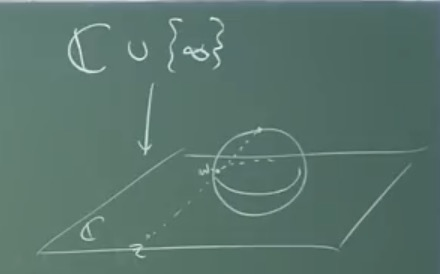
\includegraphics[scale=0.5]{RiemannSphere.jpg}
    \caption{Riemann Sphere}
    \label{RiemannSphere}
\end{figure}

The conformal group is a bit larger which is 
\begin{equation}
    \mathrm{Conf}(\mathbb{C}\cup\{\infty\})=\{f(z)|f(z)=\frac{\alpha z+\beta}{\gamma z+\delta};\quad\alpha,\beta,\gamma,\delta\in\mathbb{C}\quad\&\quad\alpha\delta-\beta\gamma\neq0\}
\end{equation}
The above group is the group of Möbius transformations.

\subsubsection{$d=2$ Case in Euclidean Space: Local Transformation}
Consider a infitesimal transformation
\begin{equation}
\begin{aligned}
z\rightarrow z+\epsilon(z)\\
\bar{z}\rightarrow \bar{z}+\bar{\epsilon}(\bar{z})
\end{aligned}
\end{equation}
where $\epsilon$ is holomorphic. For convienience , we consider the basis $\epsilon_n=-\epsilon z^{n+1}$. 

we consider the vector field corresponding to the transformation of $z\rightarrow z+\epsilon_n(z)$ by considering the diffeomorphism
\begin{equation}
    \phi[z\rightarrow z+\epsilon_n]=e^{\epsilon l_n}
\end{equation}
where $l_n\in\mathrm{T}_z\mathcal{M}=\mathrm{T}_z\mathbb{C}$. It is obvious that $l_n$ and its conjugate is of the form
\begin{equation}
\begin{aligned}
l_n=-z^{n+1}\partial_z\\
\bar{l}_n=-\bar{z}^{n+1}\partial_{\bar{z}}
\end{aligned}
\end{equation}
We have the following commutation relation between the generators $l_n$ and $\bar{l}_n$
\begin{equation}
[l_n,l_m]=(m-n)l_{m+n}
\end{equation}
\begin{equation}
    [\bar{l}_n,\bar{l}_m]=(m-n)\bar{l}_{m+n}
\end{equation}
\begin{equation}
    [\bar{l}_m,l_n]=0
\end{equation}
These generators form an infinite dimensional Lie Algebra called Witt algebra. It is obvious that Witt algebra is a direct sum of two isomorphic algebras.

Now, we are going to see which $l_n$s are corresponding to global conformal transformations. Consider a verctor field,
\begin{equation}
    V=-\sum_{-\infty}^\infty V_nl_n=\sum V_nz^{n+1}\partial_z.
\end{equation}
 Global transformation requires $V$ to exponentiate to a holomorphic map $f$ with holomorphic inverse.
 \begin{enumerate}
     \item $f$ is holomorphic means it is non-singular as $z\rightarrow0$, which tells us $V_n=0$ for $n<-1$.
     \item The inverse of $f$ is holomorphic means it is non-singular as $z\rightarrow0$ on Riemann Sphere, which tells us $V_n=0$ for $n>1$.
 \end{enumerate}
Thus the only possible choice we have are $l_{-1}$, $l_0$,$l_1$ and $\bar{l}_{-1}$,$\bar{l}_0$,$\bar{l}_1$. From the commutation relations, they are close to form a subalgebra of Witt algebra.

We claim they generate Möbius transformations by giving the correspondence between the generators and the transformations
\begin{equation*}
\begin{aligned}
e^{sl_{-1}}&=\phi[z\rightarrow z-s]\\
e^{s(l_0+\bar{l}_0)}&=\phi[z\rightarrow e^{-s}z]\\
e^{is(\bar{l}_0-l_0)}&=\phi[z\rightarrow e^{is}z]\\
e^{sl_1}&=\phi[z\rightarrow \frac{z}{1+sz}]
\end{aligned}
\end{equation*}
These four diffeomorphisms give us translation, dilation, rotation and special conformal transformation separately.

The Möbius transformation can also be expressed in matrix form by
\begin{equation}
    f_{abcd}(z)=\frac{az+b}{cz+d}\iff\begin{bmatrix}
    a&&&b\\
    c&&&d
    \end{bmatrix}
\end{equation}
The composition of the tranformation can be seen as matrix product. The composition of the transformation is given by
\begin{equation}
    f_{ekgh}\circ f_{abcd}(z)=\frac{ef_{abcd}(z)+k}{gf_{abcd}(z)+h}=\frac{(ae+ck)z+be+dk}{(ag+bh)z+bg+dh}
\end{equation}
and the matrix product is given by
\begin{equation}
    \begin{bmatrix}
    e&&k\\
    g&&h
    \end{bmatrix}
    \begin{bmatrix}
    a && b\\
    c && d
    \end{bmatrix}=\begin{bmatrix}
    ae+ck && be+dk\\
    ag+ch && bg+dh
    \end{bmatrix}.
\end{equation}
With this formulation, we can write down the matrix form for the transformations
\begin{equation}
\begin{aligned}
e^{-\beta l_{-1}}&\rightarrow\begin{bmatrix}1 &&&\beta\\0&&&1
\end{bmatrix}\\
e^{-2\ln\lambda(l_0+\bar{l}_0)}&\rightarrow\begin{bmatrix}\lambda&&&0\\0&&&\lambda^{-1}
\end{bmatrix}\\
e^{i\theta(\bar{l}_0-l_0)}&\rightarrow\begin{bmatrix}
e^{i\frac{\theta}{2}}&&&0\\0&&&e^{-i\frac{\theta}{2}}
\end{bmatrix}\\
e^{cl_1}&\rightarrow\begin{bmatrix}
1&&&0\\c&&&1
\end{bmatrix}
\end{aligned}.
\end{equation}

\subsubsection{$d=2$ Case in Minkovski Space}
The conformal group of $\mathbb{R}^{1,1}$ is special. We have the following theorem
\begin{framed}
A smooth map 
\begin{equation}
    \phi=(u,v):M\rightarrow\mathbb{R}^{1,1}
\end{equation}
from connected subset $M\subset\mathbb{R}^{1,1}$ is conformal $\iff$ $u_x^2>v_x^2$ together with the condition $u_x=v_y$, $u_y=v_x$ or $u_x=-v_y$, $u_y=-v_x$.
\end{framed}
\begin{figure}
    \centering
    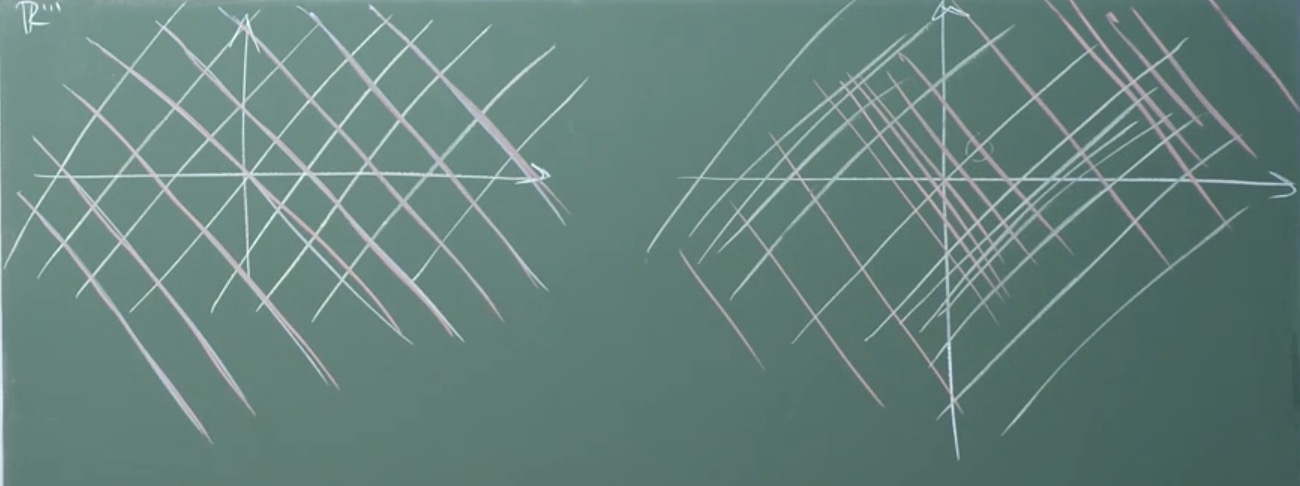
\includegraphics[scale=0.3]{dilationinR11.jpg}
    \caption{An example of conformal transformation in $\mathbb{R}^{1,1}$ in lightcone coordinate: dilation} 
\end{figure}
The following theorem captures the essence of conformal transformation in $\mathbb{R}^{1,1}$
\begin{framed}
For $f\in \mathrm{C}^\infty(\mathbb{R})$, we define $f_{\pm}\in \mathrm{C}^\infty(\mathbb{R}^2,\mathbb{R})$ by
\begin{equation*}
    f_{\pm}(x,y)=f(x\pm y).
\end{equation*}
The map $\Phi:\mathrm{C}^\infty(\mathbb{R})\times\mathrm{C}^\infty(\mathbb{R})\rightarrow \mathrm{C}^\infty(\mathbb{R}^2,\mathbb{R})^2$
\begin{equation}
    (f,g)\rightarrow\frac{1}{2}(f_++g_-,f_+-g_-)
\end{equation}
has properties
\begin{enumerate}
    \item $\mathrm{Im}\Phi=\{(u,v)|u_x=v_y\& u_y=v_x\}$.
    \item $\Phi(f,g)$ is conformal $\iff$ $f'>0$, $g'>0$ or $f'<0$, $g'<0$.
    \item $\Phi$ is bijective $\iff$ $f$ and $g$ are bijective.
    \item $\Phi(f\circ h,g\circ k)=\Phi(f,g)\circ\Phi(h,k)$ for all $f$, $g$, $h$, $k$ $\in\mathrm{C}^\infty(\mathbb{R})$
\end{enumerate}
\end{framed}
A directed result from above theorem is
\begin{framed}
Group of orientation-preserving transformations of $\mathcal{M}=\mathbb{R}^{1,1}$ is isomorphic to
\begin{equation*}
    \bigg(\mathrm{Diff}_+(\mathbb{R})\times\mathrm{Diff}_+(\mathbb{R})\bigg)\cup\bigg(\mathrm{Diff}_-(\mathbb{R})\times\mathrm{Diff}_-(\mathbb{R})\bigg)
\end{equation*}
\end{framed}
Usually, we drop the second part and only consider the first part. If we compactify $\mathbb{R}^{1,1}\rightarrow S^{1,1}\subset(\mathbb{R}^{2,0}\times\mathbb{R}^{0,2})$, we have almost the same result as
\begin{framed}
Group of orientation-preserving transformations of $\mathcal{M}=S^{1,1}$ is isomorphic to
\begin{equation*}
    \mathrm{Conf}(\mathbb{R}^{1,1})\equiv\bigg(\mathrm{Diff}_+(S^1)\times\mathrm{Diff}_+(S^1)\bigg)\cup\bigg(\mathrm{Diff}_-(S^1)\times\mathrm{Diff}_-(S^1)\bigg).
\end{equation*}
This is the definition of $\mathrm{Conf}(\mathbb{R}^{1,1})$.
\end{framed}

\newpage

\section{Classical Conformal Field Theory}
So far, we have the following correspondence 
\begin{enumerate}
    \item Conformal symmetry $\leftrightarrow$ $\mathrm{Conf}(\mathbb{R}^{p,q})$
    \item Infiitesimal conformal transformation $\leftrightarrow$ Witt algebra
\end{enumerate}

What is a conformal *theory*? A conformal theory is a theory with a representation of group $G=\mathrm{Conf}(\mathbb{R}^{p,q})$
\begin{equation*}
\begin{aligned}
\pi:&G\rightarrow M_n(\mathbb{C})\\
\pi:&G\rightarrow \mathcal{L}(\mathcal{H})
\end{aligned}
\end{equation*}
which are corresponding to finite and infinite representation explicitly.

We also want our theory to be local, which means we have a collection of observables $\phi_a(x)$ with $x\in\mathbb{R}^{p,q}$ and $a\in I$ where $I$ is the index set. A fact need to be noted is that it is likely that a representation of G has a coolection of local observables is reducible.

\subsection{Symmetries in Classical Field Theory}
Consider a theory
\begin{equation}
    S=\int\mathrm{d}^dx\mathcal{L}(\underline{\phi},\partial_\mu\underline{\phi})
\end{equation}
with $[\underline{\phi}]=\phi_a$. A symmetry transforms
\begin{equation}
\begin{aligned}
x&\rightarrow x'\\
\underline{\phi}(x)&\rightarrow\underline{\phi}'(x')=\mathcal{F}[\underline{\phi}(x)]
\end{aligned}
\end{equation}
\begin{figure}
    \centering
    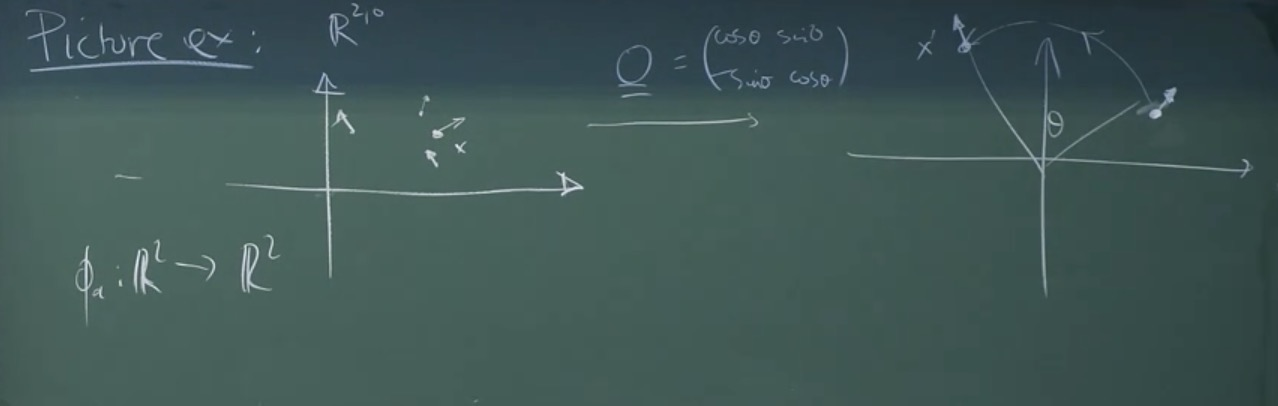
\includegraphics[scale=0.3]{2drotation.jpg}
    \caption{Rotation in 2 dimension as an example of symmetry transformation}
    \label{2drotation}
\end{figure}
An example of 2 dimensional rotation is given in Fig.(\ref{2drotation}). After the rotation, the field transforms as
\begin{equation}
    \phi_a(x)=\sum_b\pi(\underline{O})_{ab}\phi_b(\underline{O}^{-1}x).
\end{equation}
The trivial representation of $\mathrm{SO}(2)$ will give us
\begin{equation}
    \pi(\underline{O})_{ab}=\delta_{ab}
\end{equation}
and the fundamental representation gives us
\begin{equation}
    \pi(\underline{O})_{ab}=[\underline{O}]_{ab}.
\end{equation}
The irreducible representations of $\mathrm{SO}(3)$ is labelled by spin $j=0,1/2,1,...$

The new action $S'$ after above transformation is given by
\begin{equation}
    S'=\int\mathrm{d}^dx\left|\frac{\partial x'}{\partial x}\right|\mathcal{L}\bigg(\mathcal{F}(\phi(x)),\frac{\partial^{\nu}}{\partial x'^{\mu}}\partial_\nu\mathcal{F}(\phi(x))\bigg)
\end{equation}
where 
\begin{equation}
    \left|\frac{\partial x'}{\partial x}\right|=\left|\mathrm{det}(\frac{\partial x'^\mu}{\partial x^\nu})\right|.
\end{equation}
We say a theory in symmetric over the transformation if the equation of motions are invariant, i.e.
\begin{equation}
    \mathcal{L}'=\mathcal{L}+\partial M.
\end{equation}
\subsection{Facts of $\mathrm{Conf}(\mathbb{R}^{p,q})$}
With the analysis above of $\mathrm{Conf}(\mathbb{R}^{p,q})$, we can write down the infinitesimal generators
\begin{enumerate}
    \item Translation $P_\mu=-i\partial_\mu$
    \item Dilation $D=-ix^\mu\partial_\mu$
    \item Rotation $L_{\mu\nu}=i(x_\mu\partial_\nu-x_\nu\partial_\mu)$
    \item SCTs $K_\mu=-i(2x_\mu x^\nu\partial_\nu-x^2\partial_\mu)$
\end{enumerate}
We can also write down the Lie algebras
\begin{equation}
\begin{aligned}
\left[D,P_\mu\right]&=iP_\mu\\
\left[D,K_\mu\right]&=-iK_\mu\\
\left[K_\mu,P_\nu\right]&=2i(\eta_{\mu\nu}D-L_{\mu\nu})\\
\left[K_\rho,L_{\mu\nu}\right]&=i(\eta_{\rho\mu}K_{\nu}-\eta_{\rho\nu}K_\mu)\\
\left[P_\rho,L_{\mu\nu}\right]&=i(\eta_{\rho\mu}P_\nu-\eta_{\rho\nv}P_\mu)\\
\left[L_{\mu\nu},L_{\rho\sigma}\right]&=i(\eta_{\nu\rho}L_{\mu\sigma}+\eta_{\mu\sigma}L_{\nu\rho}-\eta_{\mu\rho}L_{\nu\sigma}-\eta_{\nu\sigma}L_{\mu\rho})
\end{aligned}.
\end{equation}
\subsection{Classical Conformal Field Theory}
With the knowledge above, we are going to find out what kinds of fields representaition transfrom under $\mathrm{Conf}(\mathbb{R}^{p,q})$. We already know Poincare group is a subgroup of conformal group. Then, a representation of conformal group is also a representation of Poincare group.
\begin{equation}
    \phi_a(x)\rightarrow\sum_b\pi(\Lambda)_{ab}\phi_b(\Lambda^{-1}x)
\end{equation}
where $\pi$ is some representation of Poincare group.

We focus on the subgroup of the conformal group $\mathrm{Conf}(\mathbb{R}^{p,q})$ which leave the origin fixed, i.e. boost/rotation, dilation and SCTs.

Consider a infinitesimal transformation $\Lambda=e^{i\omega^aG_a}$, where $\omega^a$ is infinitesimal and $G_a\in\{K_\mu,D,L_{\mu\nu}\}$. The field at origin transforms as
\begin{equation}
    \phi_a(0)\rightarrow\sum_b\pi(e^{i\omega^aG_a})_{ab}\phi_b(0).
\end{equation}
Since $\omega^a$ is infinitesimal, we can write
\begin{equation}
    \pi(e^{i\omega^aG_a})=\pi(1)+i\omega^a\pi(G_a).
\end{equation}
Denote
\begin{equation}
\begin{aligned}
\pi(D)&=\tilde{\Delta}\\
\pi(K_\mu)&=\kappa_\mu\\
\pi(L_{\mu\nu})&=S_{\mu\nu}
\end{aligned}
\end{equation}
The Lie algebra tell us
\begin{equation}
\begin{aligned}
\left[\tilde{\Delta},S_{\mu\nu}\right]&=0\\
\left[\tilde{\Delta},\kappa_\mu\right]&=-i\kappa_\mu\\
\left[\kappa_\mu,\kappa_\nu\right]&=0
\end{aligned}.
\end{equation}
If we suppose $S_{\mu\nu}$ is an irreducible representation of Lorentz group, with Schur's lemma, we have $\tilde{\Delta}\propto\mathds{1}$. This tells us $-i\kappa_\mu=0$. Denote $\tilde{\Delta}=i\Delta\mathds{1}$.

With above facts, we can write down how dilation acts on the field
\begin{equation}
\begin{aligned}
x&\rightarrow\lambda x=\lambda^\epsilon\lambda^\epsilon...\lambda^\epsilon x\\
\phi_a (0)&\rightarrow(\mathds{1}+i\epsilon\tilde{\Delta})(\mathds{1}+i\epsilon\tilde{\Delta})...(\mathds{1}+i\epsilon\tilde{\Delta})\phi_a(0)\\
&=\lambda^{i\tilde{\Delta_a}}\phi_a(0)=\lambda^{-\Delta_a}\phi_a(0).
\label{Dilation}
\end{aligned}
\end{equation}
This shows us every conformal field has a scaling dimension $\Delta_a$ which will actually becomes a new quantum number for quantum conformal field theory. We denote
\begin{equation}
    \Lambda=\lambda^{-2}
\end{equation}
and the Jacobian and metric under the transformation can be written as 
\begin{equation}
\begin{aligned}
g'_{\mu\nu}&=\Lambda g_{\mu\nu}\\
\left|\frac{\partial x'}{\partial x}\right|&=\Lambda^{-d/2}
\end{aligned}
\end{equation}
With this new notation, the dilation in Eq.(\ref{Dilation}) can be re-written as
\begin{equation}
    \phi(x)\rightarrow\phi'(x')=\left|\frac{\partial x'}{\partial x}\right|^{-\Delta/d}\phi(x).
\end{equation}
This is a more useful expression for dilation. Note, we generalize the result from the origin to all the space. The way we generalize it is shown as below
\begin{framed}
\begin{equation}
\begin{aligned}
    \phi_a'(x)&=\sum_b\pi(\Lambda)_{ab}\phi_b(\Lambda^{-1}x)\\
    &=\sum_b[\lambda^{-\Delta}]_{ab}\phi_b(\Lambda^{-1}x)\\
    &=\lambda^{-\Delta}\phi_a(\lambda^{-1}x)
\end{aligned}    
\end{equation}
\end{framed}

So far, we have found the representation of the subgroup preserves the origin. In order to find the representation anywhere, we can use the translation operator to translate the generators to $x$, by
\begin{equation}
\begin{aligned}
    e^{ix^\rho P_\rho}De^{-x^\rho P_\rho}&=D+x^\rho P_\rho\\
    e^{ix^\rho P_\rho}S_{\mu\nu}e^{-x^\rho P_\rho}&=S_{\mu\nu}-(x_\mu P_\nu-x_\nu P_\mu)
\end{aligned}
\end{equation}

\newpage
\section{Quantum Conformal Field Theory}
A quantum field theory is a quantum theory. Thus, we need the following data to construct a quantum conformal field theory
\begin{itemize}
    \item Hilbert Space $\mathcal{H}$
    \item Projective unitary representation of the symmetry group
    \item Vacuum: $|0\rangle\in\mathcal{H}$ is invariant under the global conformal symmetry up to a phase.
    \item Observables: $A_{j}(x)$ where $x\in\mathrm{R}^{p,q}$ and $j$ labels particle types etc.
\end{itemize}

Before we begin to talk about a quantum conformal field theory, we have the following definition:
\begin{framed}
A quasi-primary operators are a subset of {$A_j(x)$|$x\in\mathrm{R}^{p,q}$}, denoted by ${\hat{\phi}_k(x)|k\in K}$ such that 
\begin{equation*}
    \hat{\phi}_k(x)\xrightarrow{U(g)}\left|\frac{\partial x'}{\partial x}\right|^{\Delta_k/d}\hat{\phi}'_k(x')=U^\dagger(g)\hat{\phi}_k(x)U(g)
\end{equation*}
where $x'=gx$.
\end{framed}
\subsection{Quantum Field Theory with Global Conformal Symmetry}
From the definition, we can write down the constraints for the n-point function of a quasi-primary field
\begin{equation}
    \langle\phi_{k_1}(x_1)...\phi_{k_n}(x_n)\rangle=\left|\frac{\partial x'_1}{\partial x_1}\right|^{\Delta_{k_1}/d}...\left|\frac{\partial x'_n}{\partial x_n}\right|^{\Delta_{k_n}/d} \langle\phi'_{k_1}(x'_1)...\phi'_{k_n}(x'_n)\rangle
\label{constraints on n-point function}
\end{equation}

We then look at the invariants of conformal group
\begin{itemize}
    \item Translation: $x_i,x_j\in\mathrm{R}_{p,q}$, $x_i-x_j$ is invariant. We have $d(N-1)$ independent quantities.
    \item Rotation: for spinless objects $r_{ij}=\left|x_i-x_j\right|$ is invariant. We have $N(N-1)/2$ totally.
    \item Scale invariance: $\frac{r_{ij}}{r_{mn}}$
    \item SCTs: cross ratio $\frac{r_{ij}r_{mn}}{r_{im}r_{jn}}$ is invariant.
\end{itemize}
\vspace{3in}

Let's now look at a 2-point function specifically. For a 2-point function, we have \begin{equation}
     \langle\phi_{1}(x_1)\phi_{2}(x_2)\rangle=\left|\frac{\partial x'_1}{\partial x_1}\right|^{\Delta_{1}/d}\left|\frac{\partial x'_2}{\partial x_2}\right|^{\Delta_{2}/d} \langle\phi'_{1}(x'_1)...\phi'_{2}(x'_2)\rangle
\end{equation}
\begin{itemize}
    \item The translation and rotation symmetry told us the LHS only depends on $r_{12}=\left|x_1-x_2\right|$, i.e. $G(x_1,x_2)=f(r_{12})$ for some function $f$.
    \item Under dilations
    \begin{equation*}
        f(r_{12})=\lambda^{\Delta_1+\Delta_2}f(\lambda r_{12}).
    \end{equation*}
    This tells us $f$ is of the form 
    \begin{equation*}
        f(r_{12})=\frac{C_{12}}{r_{12}^{\Delta_1+\Delta_2}}
    \end{equation*}
    \item Under SCTs
    \begin{equation}
        \langle\phi_1(x_1)\phi_2(x_2)\rangle=\left\{\begin{aligned}\frac{C_{12}}{r_{12}^{2\Delta}}&&\Delta_1=\Delta_2=\Delta\\0 &&\mathrm{otherwise}
    \end{aligned}\right.\end{equation}
\end{itemize}

For 3-point function, with the same analysis, we have
\begin{itemize}
    \item From translation, rotation and dilation symmetry
    \begin{equation*}
        \langle\phi_1(x_1)\phi_2(x_2)\phi_3(x_3)\rangle=\sum_{a,b,c}\frac{C_{abc}}{r_{12}^ar_{23}^br_{13}^c}
    \end{equation*}
    where $a+b+c=\Delta_1+\Delta_2+\Delta_3$
    \item Under SCTs 
    \begin{equation*}
        \begin{aligned}
            a&=\Delta_1+\Delta_2-\Delta_3\\
            b&=\Delta_2-\Delta_1+\Delta_3\\
            c&=\Delta_1-\Delta_2+\Delta_3
        \end{aligned}
    \end{equation*}
    so
    \begin{equation*}
        \langle\phi_1(x_1)\phi_2(x_2)\phi_3(x_3)\rangle=\frac{C_{123}}{r_{12}^{\Delta_1+\Delta_2-\Delta_3}r_{23}^{\Delta_2-\Delta_1+\Delta_3}r_{13}^{\Delta_1-\Delta_2+\Delta_3}}
    \end{equation*}
\end{itemize}

With the same idea, the 4-point function can be written as
\begin{equation}
    G^{(4)}(x_1,x_2,x_3,x_4)=F(\frac{r_{12}r_{34}}{r_{13}r_{24}},\frac{r_{12}r_{34}}{r_{14}r_{23}})\prod_{j<k}r_{jk}^{\Delta/3-(\Delta_j+\Delta_k)}
\end{equation}
where $F(x,y)$ is an arbitrary function and $\Delta=\sum\Delta_j$
\subsection{Conformal Theory in (2+0) Dimension}
We defined 
\begin{equation}
\begin{aligned}
    z=x+iy\\
    \bar{z}=x-iy
\end{aligned}
\end{equation}
We assumed that we can analytically continue to arbitrary $z$ and $\bar{z}$ with
\begin{equation}
\Phi(x,y)=\Phi(z,\bar{z}).
\end{equation}
We have the following definition in a 2-d conformal field theory
\begin{framed}
A primary operator with conformal wright $(h,\bar{h})$ is a field transforming in the following way
\begin{equation*}
    \Phi(z,\bar{z})=\bigg(\frac{\partial f}{\partial z}\bigg)^h\bigg(\frac{\partial\bar{f}}{\partial\bar{z}}\bigg)^{\bar{h}}\Phi\big(f(z),\bar{f}(\bar{z})\big)
\end{equation*}
\end{framed}

Infinitesimally, we can write above definition as 
\begin{equation}
    \delta_{\epsilon,\bar{\epsilon}}\Phi(z,\bar{z})=\bigg((h\partial\epsilon+\epsilon\partial)+(\bar{h}\bar{\partial}\bar{\epsilon}+\bar{\epsilon}\bar{\partial})\bigg)\Phi(z,\bar{z})
\end{equation}
where $f(z)=z+\epsilon(z)$. 

We consider the 2-point function first
\begin{equation}
    G^{(2)}(z_1,\bar{z}_1;z_2,\bar{z}_2)=\langle\Phi_1(z_1,\bar{z}_1)\Phi_2(z_2,\bar{z}_2)\rangle.
\end{equation}
With the infinitesimal transformation, we have
\begin{equation}
    0=\delta_{\epsilon,\bar{\epsilon}}G^{(2)}
    (z_1,\bar{z}_1,z_2,\bar{z}_2)=\langle\delta_{\epsilon,\bar{\epsilon}}\Phi_1\Phi_2\rangle+\langle\Phi_1\delta_{\epsilon,\bar{\epsilon}}\Phi_2\rangle
\end{equation}
\begin{itemize}
    \item $\epsilon(z)=\epsilon$: we have $G^{(2)}$ only depends on $z_{12}=z_1-z_2$
    \item $\epsilon(z)=\epsilon z$: we have $G^{(2)}=\frac{C_{12}}{z_{12}^{h_1+h_2}\bar{z}_{12}^{\bar{h}_1+\bar{h}_2}}$
    \item $\epsilon(z)=z^2$: we have $G^{(2)}=\frac{C_{12}}{z_{12}^{2h}\bar{z}_{12}^{2\bar{h}}}$
\end{itemize}
With above 3 constraints, we can write
\begin{equation}
    G^{(2)}(z_1,\bar{z}_1,z_2,\bar{z}_2)=\frac{C_{12}}{z_{12}^{2h}\bar{z}_{12}^{2\bar{h}}}
\end{equation}
If we have a bosonic field with $h=\bar{h}$, we return back to the result we obtained for global conformal symmetry
\begin{equation}
    G^{(2)}(z_1,\bar{z}_1,z_2,\bar{z}_2)=\frac{C_{12}}{\left|z_{12}\right|^{2\Delta}}
\end{equation}
where $\Delta=h+\bar{h}$

\newpage
\subsection{Ward Identity}
\subsubsection{General form}
Suppose we have a tuple of fields $\Phi(x)$ and action $S$. Let $S$ be invariant under the symmetry transformation
\begin{equation}
    \Phi'(x)=\Phi(x)-i\omega_a\hat{G}_a\Phi(x)
\end{equation}
where $G_a$ is the generator of the Lie algebra, i.e.
\begin{itemize}
    \item Dilation: $G_a=-ix^\nu\partial_\nu-i\Delta_a$
    \item Translation: $G_a=-i\partial_\nu$
    \item ...
\end{itemize}
We look at the n-point function
\begin{equation}
    \hat{X}=\hat{\Phi(x_1)}...\hat{\Phi(x_n)}
\end{equation}
with path integral formulation
\begin{equation}
    \langle\hat{X}\rangle=\frac{1}{Z}\int\mathcal{D}\Phi\hat{X}e^{-S}
\end{equation}
in Euclidean Space. We make the assumption here that after the symmetry transformation, the path integral measure keeps the same, i.e.
\begin{equation}
    \mathcal{D}\Phi'=\mathcal{D}\Phi.
\end{equation}
This is a nontrivial assumption since we assume we have no anomaly in the symmetry we are considering.

The n-point function in the action after symmetry transformation reads
\begin{equation}
    \langle\hat{X}\rangle=\frac{1}{Z}\int\mathcal{D}\Phi'(\hat{X}+\delta\hat{X})e^{-S[\Phi]+\int\mathrm{d}^dx\partial_\mu j^{\mu}_a\omega_a(x)}
\end{equation}
We have to the first order in $\omega$,
\begin{equation}
    \delta\hat{X}=-i\sum_{j=1}^n\omega_a(x_j)\bigg(\hat{\Phi}(x_1)...\hat{G}_a\hat{\Phi}_(x_j)...\hat{\Phi}(x_n)\bigg)
\end{equation}
Since the value of the n-point function should be independent over the representation of the field, by comparing Eq.(4.14) and Eq.(4.16), we have to the first order of $\omega$
\begin{equation}
    \langle\delta\hat{X}\rangle=\int\mathrm{d}^dx\partial_\mu\langle\hat{j}^{\mu}_a\hat{X}\rangle\omega_a(x).
\end{equation}
By taking $\omega_a(x)$ in a form of Dirac delta function $\omega_a(x)=\delta(x-x_0)$, we finally have the Ward identity writes
\begin{equation}
    \partial_\mu\langle\hat{j}_a^{\mu}(x)\hat{X}\rangle=-i\sum_{j=1}^n\delta(x-x_j)\langle\hat{\Phi}(x_1)...\hat{G}_a\hat{\Phi}(x_j)...\hat{\Phi}(x_n)\rangle
\end{equation}
We can integrate over all spacetime on $x$ and the LHS should be $0$. For the RHS, we obtains
\begin{equation}
    \delta_\omega\langle\hat{X}\rangle=-i\omega_a\sum_{j=1}^n\delta(x-x_j)\langle\hat{\Phi}(x_1)...\hat{G}_a\hat{\Phi}(x_j)...\hat{\Phi}(x_n)\rangle=0
\end{equation}
For the conserved charge, we have
\begin{equation}
    \hat{Q}_a=\int\mathrm{d}^{d-1}x\hat{j}_a^0(x).
\end{equation}
It corresponds to a generator. To see that, we integrate the Ward identity over a thin box $t_-<x_0<t_+$ instead of the whole spacetime. We assume $x_1^0$ is in the thin box and all other events in $\hat{X}$ are not in the box. The equation after integration reads
\begin{equation}
    \langle\hat{Q}_a(t_+)\hat\Phi(x_1)...\rangle-\langle\hat{\Phi}(x
    _1)\hat{Q}_-(t_-)...\rangle=-i\langle\hat{G}_a\hat{\Phi}(x_1)...\rangle
\end{equation}
Suppose $x_j^0<x_1^0$, by taking the limit $t_-\rightarrow t_+$, we finally have
\begin{equation}
    \langle[\hat{Q}_a,\hat{\Phi}(x_1)]..\rangle=-i\langle\hat{G}_a\hat{\Phi}(x_1)...\rangle
\end{equation}
Since we can put arbitrary operators in $...$, we can write down
\begin{equation}
    [\hat{Q}_a,\hat{\Phi}]=-i\hat{G}_a\hat{\Phi}
\end{equation}
To further understand the above result, we consider a translation in which
\begin{equation}
    \Phi'(x)=\Phi(x)-\epsilon^\mu\partial_\mu\Phi(x)
\end{equation}
with
\begin{equation}
  \hat{G}=i\partial_\mu  
\end{equation}
which tells us that $\hat{Q}_\mu$ is the total momentum operator $\vec{P}_\mu$.
\subsection{Wald Identities for Global Conformal Symmetries}
We consider the Ward identities for global conformal symmetry in this section.

For translation symmetry, the ward identity writes
\begin{equation}
    \partial_\mu\langle\hat{T}^\mu_\nu\hat{X}\rangle=-\sum\delta(x-x_j)\partial_{x_j^\nu}\langle\hat{X}\rangle
\end{equation}
where $\hat{T}_{\mu\nu}$ is the energy-momentum tensor, conserved current of translations $x\rightarrow x+\epsilon$. Classically, we have
\begin{equation}
    \partial^\mu T_{\mu\nu}=0.
\end{equation}
We also assume the energy momentum tensor is symmetric $T_{\mu\nu}=T_{\nu\mu}$ and traceless $T^\mu_\mu=0$. The tracelessness in nontrivial. But we can always introduce some term into the energy-momentum tensor to make it traceless and do not spoil it.

For rotation symmetry, the conserved current writes
\begin{equation}
    \hat{J}^{\mu\nu\rho}=T^{\mu\nu}x^\rho-T^{\mu\rho}x^\nu,
\end{equation}
and the Ward identity writes
\begin{equation}
    \langle(\hat{T}^{\rho\nu}-\hat{T}^{\nu\rho}\hat{X})=-i\sum\delta(x-x_j)S^{\nu\rho}_j\langle\hat{X}\rangle
\end{equation}
where $S^{\nu\rho}_j$ is the spin representation of field $j$.

For dilation, we have the generator 
\begin{equation}
    \hat{G}=\hat{D}=ix^\mu\partial_\mu-i\Delta.
\end{equation}
The conserved current can be written as
\begin{equation}
    j^\mu=T^{\mu}_\nu x^\nu.
\end{equation}
Thus, the Ward identity writes
\begin{equation}
    \langle\hat{T}^\mu_\mu\hat{X}\rangle=-\sum_j\delta(x-x_j)\Delta_j\langle\hat{X}\rangle
\end{equation}
% The bibliography will probably be heavily edited during typesetting.
% We'll parse it and, using the arxiv number or the journal data, will
% query inspire, trying to verify the data (this will probalby spot
% eventual typos) and retrive the document DOI and eventual errata.
% We however suggest to always provide author, title and journal data:
% in short all the informations that clearly identify a document.
\newpage
\begin{thebibliography}{99}




% Please avoid comments such as "For a review'', "For some examples",
% "and references therein" or move them in the text. In general,
% please leave only references in the bibliography and move all
% accessory text in footnotes.

% Also, please have only one work for each \bibitem.


\end{thebibliography}
\end{document}
